\documentclass{ikpKoeln}
\usepackage{graphicx}
\usepackage{physics}
\usepackage{xcolor}
\usepackage{tikz}
\usepackage{siunitx}
\usepackage[font=scriptsize,skip=0pt]{caption}
\usetikzlibrary{math, shapes.geometric, arrows, positioning}

\scTitle{An overview of data calibration algorithms of NeuLAND\\ in the R$^3$B setup}
\scAuthor{*}{Yanzhao}{Wang}{1}
\scAuthor{}{Paula}{Ulrich}{1}
\scAuthor{}{Igor}{Gasparic}{2}
\scAuthor{}{Andreas}{Zilges}{1}
\scAffiliation{1}{University of Cologne, Institute for Nuclear Physics, Germany}
\scAffiliation{2}{GSI Helmholtzzentrum für Schwerionenforschung, Germany}

\scTitleShort{Data calibration algorithms of NeuLAND}

\date{\scriptsize HK 44.4 \\DPG-Frühjahrstagung\\Cologne 2025 \\ \vspace{1em} Supported by BMBF (05P21PKFN1)}

\graphicspath{{../figures/}}

\addbibresource{reference.bib}

\AtBeginDocument{\RenewCommandCopy\qty\SI}

\begin{document}

{
\usebackgroundtemplate{%
	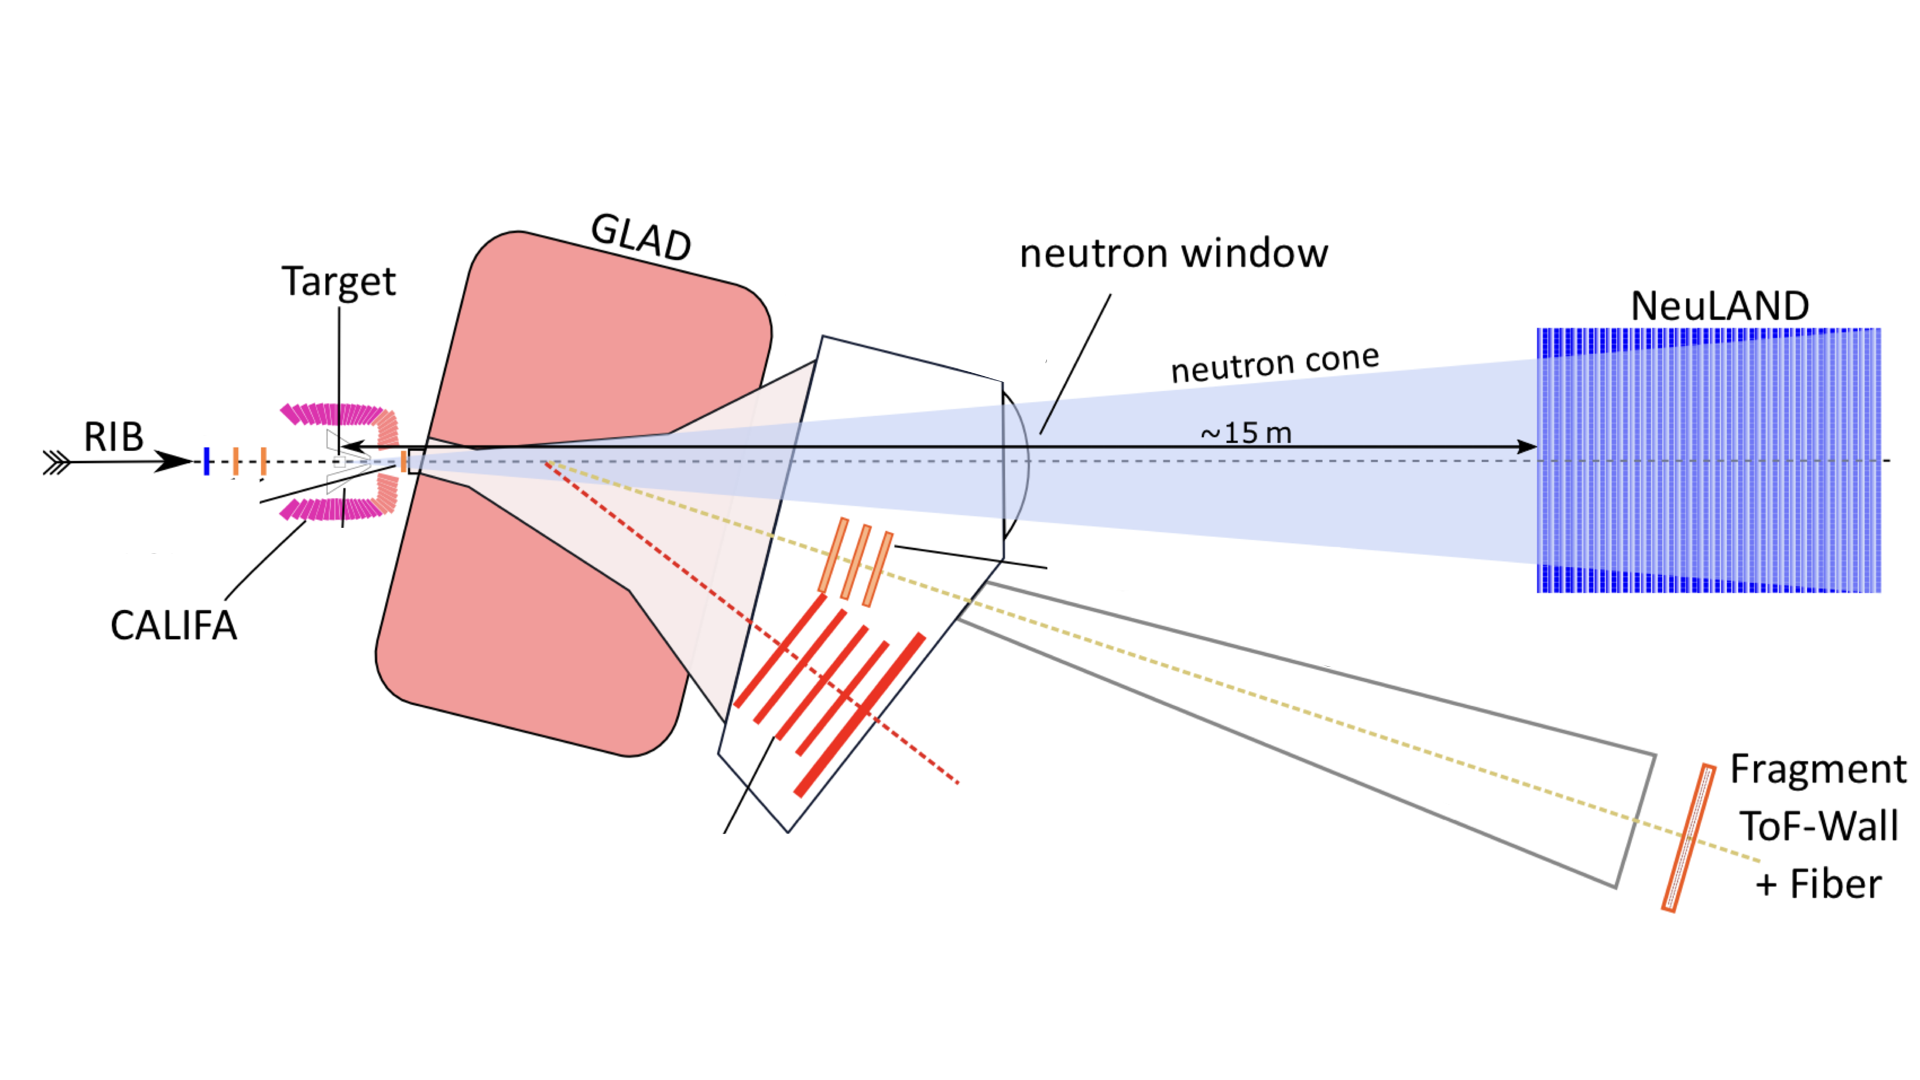
\includegraphics[width=\paperwidth, height=\paperheight]{r3b/r3bsetup_empty.png}}
\begin{frame}{NeuLAND setup in $\text{R}^3\text{B}$}

	\begin{columns}[c]
		\begin{column}{0.4\textwidth}
			\pause
			\begin{figure}
				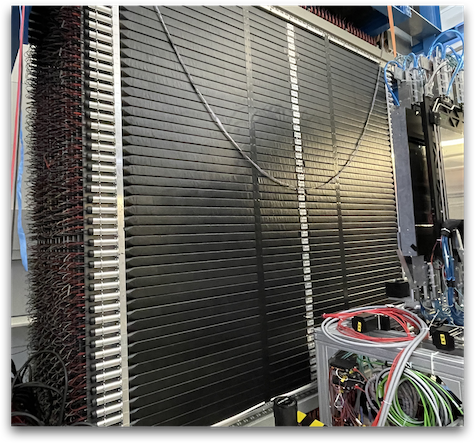
\includegraphics[width = \textwidth]{neuland/neulandReal}
			\end{figure}
		\end{column}
		\hspace*{0.5cm}
		\begin{column}{0.3\textwidth}
			\begin{exampleblock}{}
				Geometry:\\
				\begin{itemize}
					\item $26$ planes
					\item $\qtyproduct[product-units=power]{250 x 250}{\centi\meter}$
					\item $50$ scintillators each plane
					\item $2600$ PMTs in total
				\end{itemize}
				\pause
				Measurements:\\
				\begin{itemize}
					\item \alert<+(1)>{\textbf<.(1)>{interaction position}}
					\item \alert<.(1)>{\textbf<.(1)>{interaction time}}
					\item energy deposition
				\end{itemize}
			\end{exampleblock}
		\end{column}
		\begin{column}{0.3\textwidth}
		\end{column}
	\end{columns}
	\let\thefootnote\relax\footnotetext{\fullcite{BORETZKY}}
\end{frame}
}

\begin{frame}[t]{Processes of digitization}
	\begin{columns}
		\begin{column}{0.4\textwidth}
			\hspace*{-1.5em}\textbf{\textit{Physical interactions}}:
			\begin{figure}[t]
				\hspace*{-5em}
				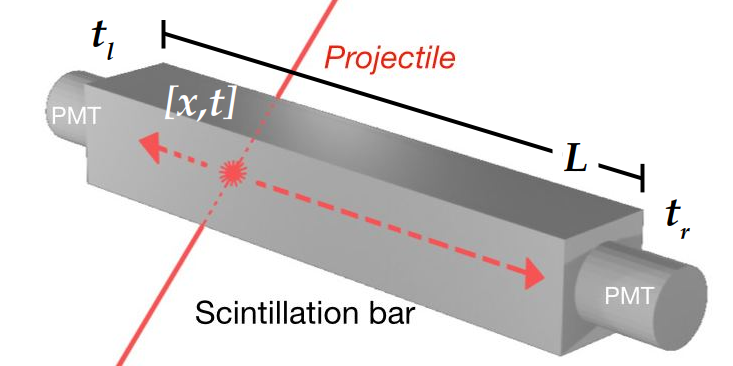
\includegraphics[width = 0.8\textwidth]{R3BCon2024GSI/Bar.png}
			\end{figure}
			\vspace{1em}
			\hspace*{-1.5em}\textbf{\textit{Digitization of PMT signals}}:
			\begin{figure}
				\hspace*{-5em}
				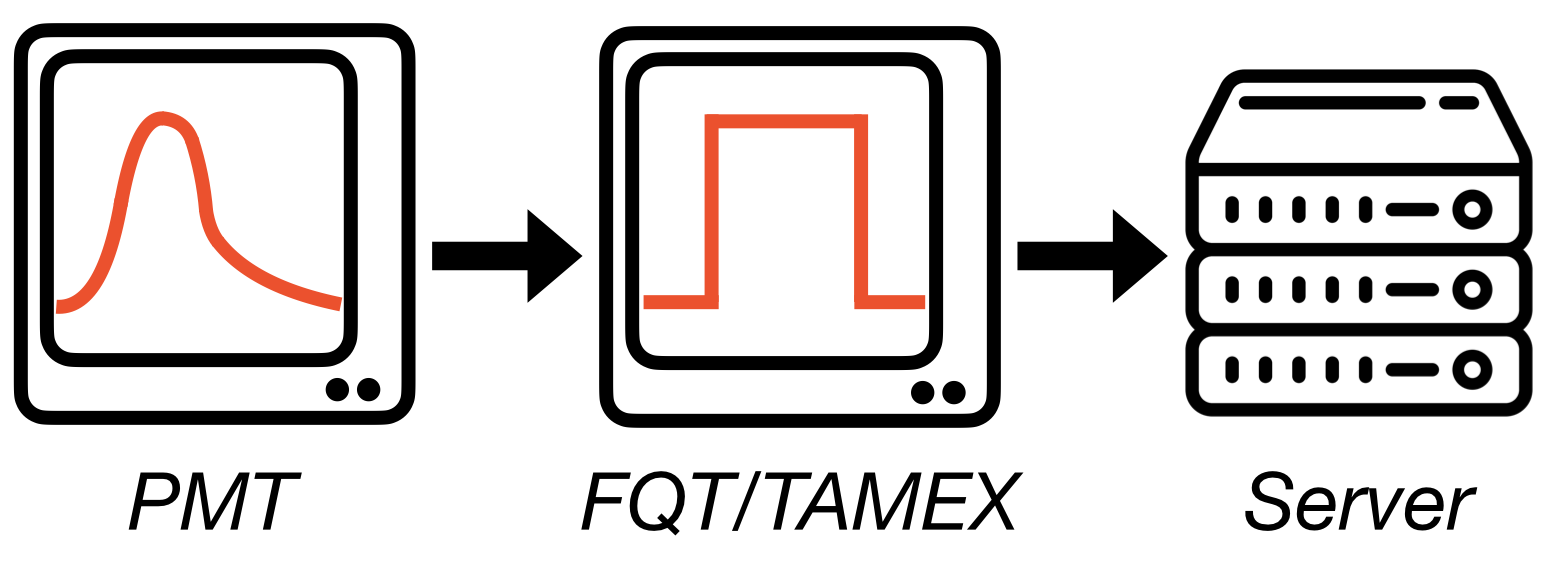
\includegraphics[width = 0.8\textwidth]{neuland/PMT2TAMEX}
			\end{figure}
		\end{column}
		\begin{column}{0.5\textwidth}
			\def\largeWidth{7cm}
			\def\smallWidth{2.5cm}
			\hspace*{-2em}
			\begin{tikzpicture} [node distance=2cm]
				\tikzstyle{lineWidth} = [line width = 0.5mm]
				\tikzstyle{dataformat} = [rectangle, rounded corners, minimum width=\largeWidth, minimum height=0.7cm, text centered, draw = black, lineWidth];
				\tikzstyle{process} = [ellipse, minimum width=3cm, minimum height=0.7cm, text centered, draw = red, lineWidth];
				\tikzstyle{arrow} = [thick, ->, >=stealth]

				\node (physical)[dataformat]{Physical data (energy, time and position)};
				\node (pmt)[process, below left =1cm and -\smallWidth of physical]{PMT, FQT};
				\node (signal)[dataformat, below = 2.5cm of physical,]{Signals (leading and trailing edges)};
				\node (tamex)[process, below left =1cm and -\smallWidth of signal]{TAMEX};
				\node (second-cal)[process, inner sep = 0mm, below right =1cm and -\smallWidth of physical, xshift = -1.5em]{2nd calibrations};
				\node (tdc)[process, inner sep = 0mm, below right =1cm and -\smallWidth of signal, xshift=-1.5em]{1st calibration};
				\node (TDCData)[dataformat, below = 2.5cm of signal]{TDC (channels, module IDs, etc)};

				\draw [arrow] (pmt.north |- physical.south) -- (pmt.north);
				\draw [arrow] (second-cal.north) -- (second-cal.north |- physical.south);
				\draw [arrow] (pmt.south) -- (pmt.south |- signal.north);
				\draw [arrow] (second-cal.south |- signal.north) -- (second-cal.south);
				\draw [arrow] (tamex.north |- signal.south) -- (tamex.north);
				\draw [arrow] (second-cal.south |- tdc.north) -- (second-cal.south |- signal.south);
				\draw [arrow] (tamex.south) -- (tamex.south |- TDCData.north);
				\draw [arrow] (second-cal.south |- TDCData.north) -- (second-cal.south |- tdc.south);

				\draw [dashed, ->, >=stealth](physical.west) -- ([xshift=-0.5em]physical.west) -- node[above, rotate = 90]{\textit{Data digitization}}([xshift=-0.5em]TDCData.west) -- (TDCData.west);
				\draw [dashed, ->, >=stealth](TDCData.east) -- ([xshift=0.6em]TDCData.east) -- node[above, rotate = -90]{\textit{Data calibration}}([xshift=0.6em]physical.east) -- (physical.east);
			\end{tikzpicture}
		\end{column}
	\end{columns}
\end{frame}

\begin{frame}[t]{Time measurement and TDC calibration}
	\vspace{-0.8em}
	\begin{columns}
		\begin{column}{0.45 \textwidth}
			\def\upperHeight{1.5cm}
			\def\lowerHeight{1cm}
			\def\totalWidth{5cm}
			\def\clockWidth{10mm}
			\def\clockHight{9mm}
			\def\signalPos{33mm}
			\def\CTHeight{-5mm}

			\textbf{\textit{Time measurement with clocks:}}
			\begin{tikzpicture}
				\draw [<-, >=stealth](0, \upperHeight) node[above, rotate=90]{\textit{\scriptsize CLK}}-- (0, -\lowerHeight);
				\draw [->, >=stealth](0, 0) -- node[very near end, below]{\scriptsize time}(\totalWidth, 0);

				\draw[thick] (0,0)
				\foreach \x in {1,...,2}{
						-- ++(0,\clockHight) -- ++(\clockWidth, 0) -- ++(0,-\clockHight) -- ++(\clockWidth,0)
					} -- ++(0,\clockHight) -- ++(\clockWidth, 0);
				\draw[thick, dashed] (\signalPos, \upperHeight) -- node[left, very near start, yshift = 1em]{trigger}(\signalPos, -\lowerHeight);
				\draw[thick, ->, >=stealth, red] (0, \CTHeight) -- node[below]{Coarse time} (40mm, \CTHeight);
				\draw[thick, <->, >=stealth, red] (\signalPos, -\CTHeight) -- node[above, yshift = 1.3em, xshift = 1.2em, name=fineTime]{Fine time} (40mm, -\CTHeight);
				\draw[red]({0.5*\signalPos + 20mm}, -\CTHeight) -- ([xshift=-1em]fineTime.south);
				\draw[thick, red] (40mm, {\CTHeight+1mm}) -- (40mm, {\CTHeight-1mm});
			\end{tikzpicture}

			\textbf{\textit{Real time calculation:}}

			\vspace{-0.5em}
			$$T_\text{real} = T_\text{coarse} - T_\text{fine}$$
			\vspace{-1em}
			\small
			{
				\begin{itemize}
					\item $T_\text{real}$: Time value relative to START detector.
					\item $T_\text{coarse}$: Clock cycles with frequency of $\qty{200}{\MHz}$
					\item $T_\text{fine}$: Fine channel numbers (TDL).
				\end{itemize}
			}
		\end{column}
		\begin{column}{0.5 \textwidth}
			\begin{figure}
				\captionsetup{labelformat=empty}
				\vspace{-0.8em}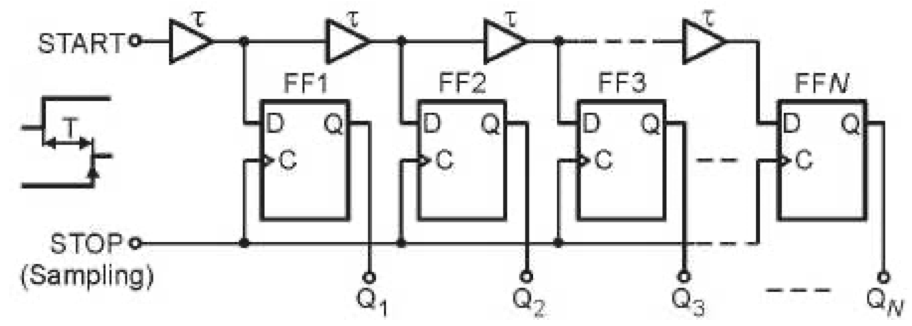
\includegraphics[width = \textwidth]{r3b/TDCFineTime}
				\caption{\scriptsize Tapped Delay Line (TDL)\footcite{TDCFINETIME}.}
				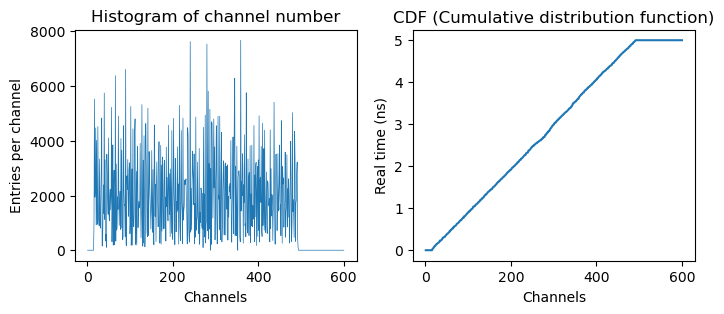
\includegraphics[width = \textwidth]{neuland/FineTimeCal}
				\caption{\scriptsize TDC Calibration (Time resolution $\sim \qty{10}{\pico\second}$).}
			\end{figure}
			\vspace*{-1.5em}
		\end{column}
	\end{columns}
\end{frame}

\begin{frame}[t]{Position, time and energy calibration parameters}
	\vspace*{-1em}
	\begin{columns}
		\begin{column}{0.4 \textwidth}
			\begin{figure}[t]
				\centering
				\vspace*{-0.5em}
				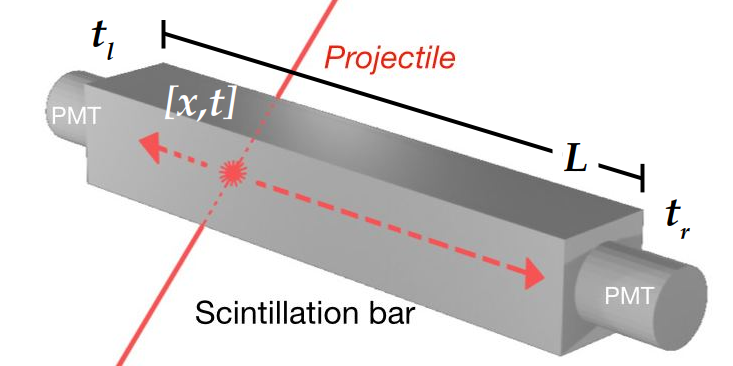
\includegraphics[width = \textwidth]{R3BCon2024GSI/Bar.png}
				\captionsetup{singlelinecheck=off,font=footnotesize}
				\vspace*{0.5em}
				\caption*{\textit{PMT saturation effect\footnotemark:}}
				\vspace*{-1em}
				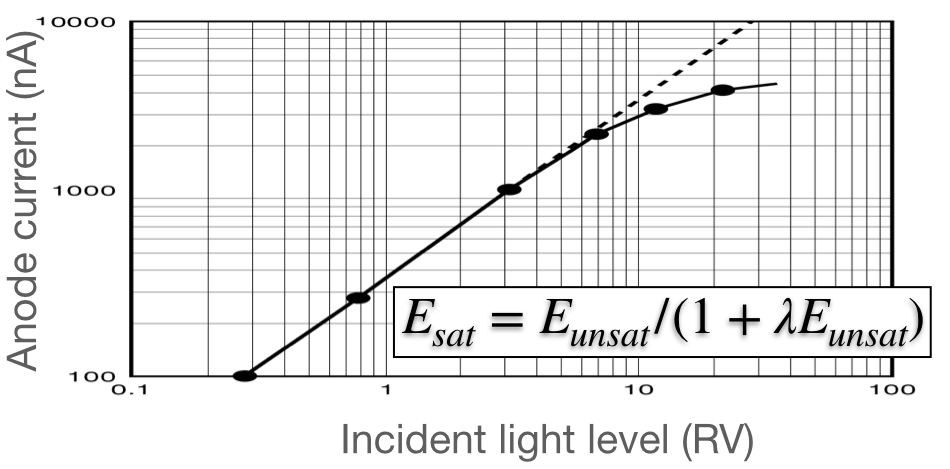
\includegraphics[width = \textwidth]{neuland/PMTSAT.png}
			\end{figure}
			\tiny{[1] \fullcite{Hamamatsu}}
		\end{column}
		\begin{column}{0.48 \textwidth}
			\vspace{-1.5em}
			\begin{block}{\small Position-Time calibration:}
				\footnotesize{
					\setlength{\abovedisplayskip}{0pt}
					\setlength{\belowdisplayskip}{0pt}
					\setlength{\abovedisplayshortskip}{0pt}
					\setlength{\belowdisplayshortskip}{0pt}
					\begin{flalign*}
						\intertext{Interaction time:}
						t & = \frac{t_r + t_l}{2} - \frac{L}{2 \cdot \alert{C_e}} + \alert{t_\text{sync}} \\
						\intertext{Interaction position:}
						x & = \frac{\alert{C_e}}{2}\left( t_r - t_l  + \alert{t_\text{offset}} \right)
					\end{flalign*}
				}
			\end{block}
			\vspace{-0.5em}
			\begin{alertblock}{\small Energy calibration:}
				\footnotesize{
					\setlength{\abovedisplayskip}{0pt}
					\setlength{\belowdisplayskip}{0pt}
					\setlength{\abovedisplayshortskip}{0pt}
					\setlength{\belowdisplayshortskip}{0pt}
					\begin{flalign*}
						\intertext{Light attenuation effect:}
						I_\text{PMT} & = E_\text{dep} \cdot \exp(-\alert{\alpha} \cdot l)     \\
						\intertext{PMT gain:}
						W            & = \alert{\mathcal{G}} \cdot I_\text{PMT} + \alert{A_0} \\
						\intertext{PMT saturation:}
						W_\text{sat} & = W \cdot / \left( 1 + \alert{\lambda} \cdot W \right)
					\end{flalign*}
				}
			\end{alertblock}
		\end{column}
	\end{columns}
\end{frame}

\begin{frame}[t]{Current position calibration}
	\vspace*{-2em}
	\begin{columns}[t]
		\begin{column}{0.45 \textwidth}
			\begin{figure}[t]
				\includegraphics<1>[width = \textwidth]{R3BCon2024GSI/side_view1.png}
				\includegraphics<2>[width = \textwidth]{R3BCon2024GSI/side_view2.png}
				\includegraphics<3-5>[width = \textwidth]{R3BCon2024GSI/side_view3.png}
				\includegraphics<6>[width = \textwidth]{R3BCon2024GSI/side_view4.png}
			\end{figure}
		\end{column}
		\begin{column}{0.45 \textwidth}
			\begin{exampleblock}{\small Procedures}
				\small
				\begin{enumerate}
					\setlength\itemsep{0em}
					\small
					\item<1-> Obtain the positions of bars with signals
					\item<2-> Reconstruct the muon track from the bar positions
					\item<3-> Calculate the positions of the interaction points of the muon
					\item<4-> Calculate the calibration parameters via data fitting
				\end{enumerate}
			\end{exampleblock}
			\onslide<5->{
				\vspace*{-0.5em}

				\textit{\small Data fitting in the position calibration:}\par
				\vspace*{-0.5em}

				\begin{figure}[t]
					\centering
					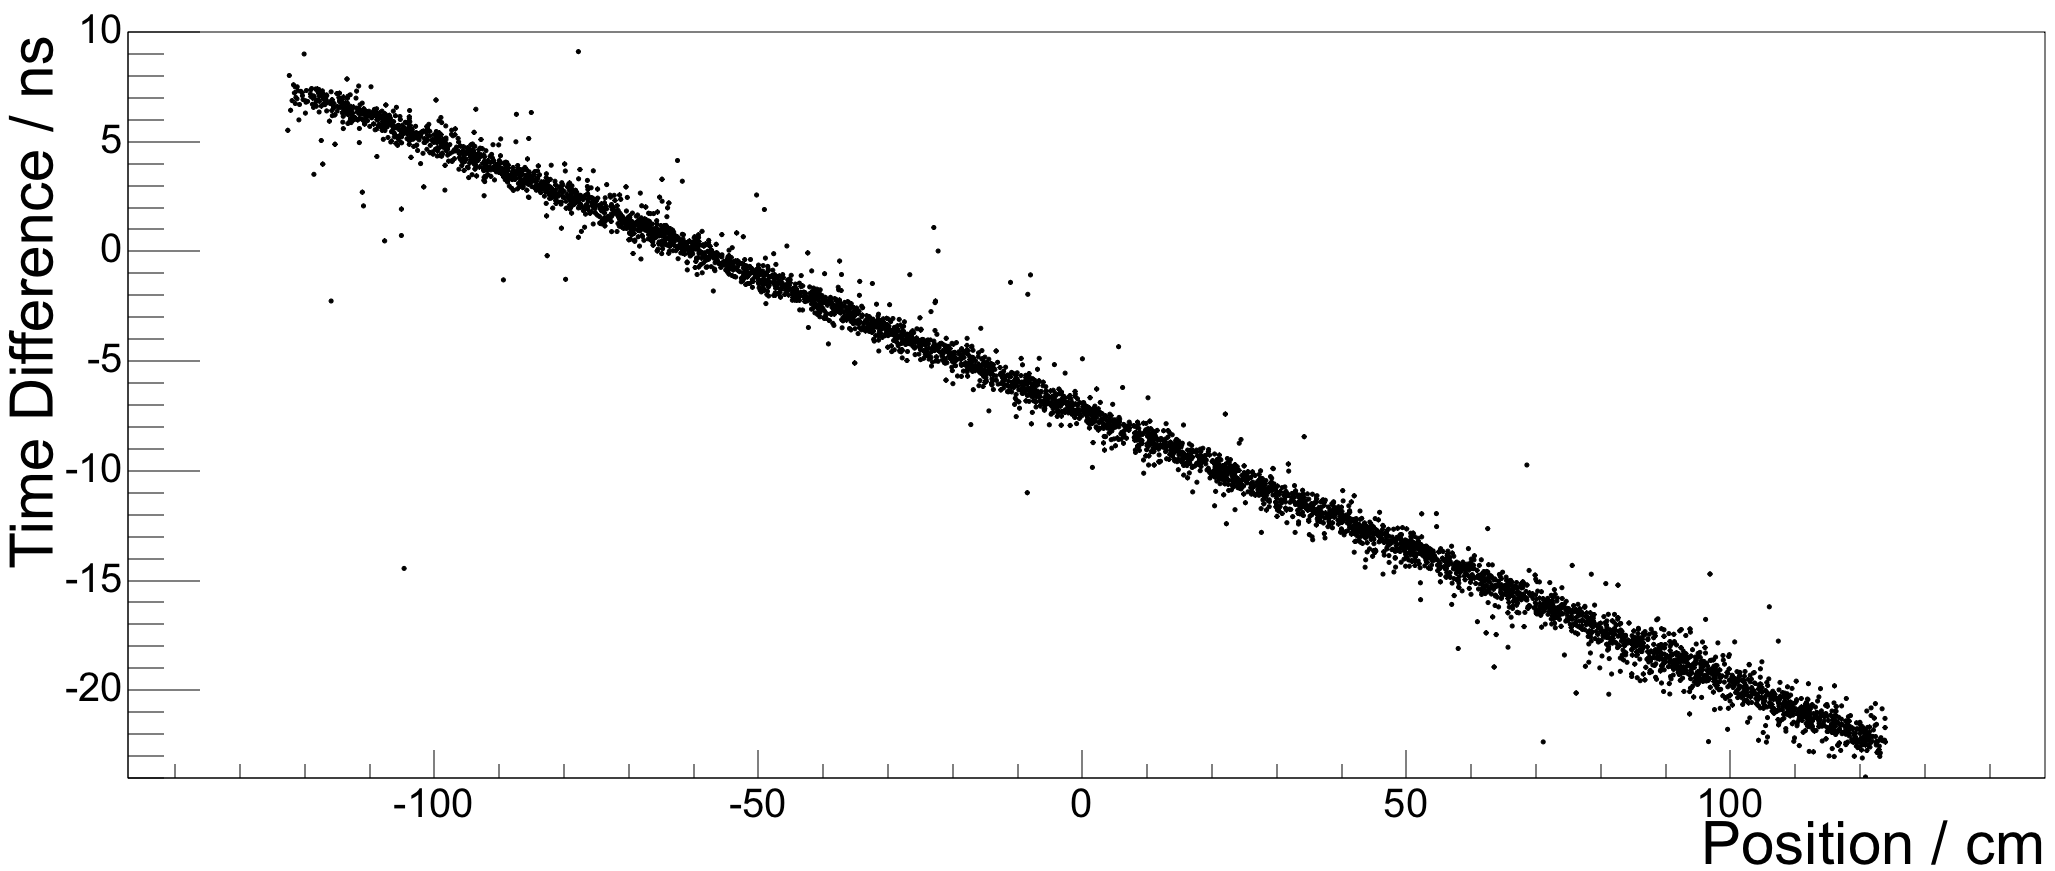
\includegraphics[ width = \textwidth]{R3BCon2024GSI/time_cal.png}
				\end{figure}
			}
		\end{column}
	\end{columns}
\end{frame}

\begin{frame}[t]{New position calibration}
	\vspace {-2em}
	\begin{columns}[t]
		\begin{column}{0.45 \textwidth}
			\begin{figure}
				\captionsetup{singlelinecheck=off,font=footnotesize}
				\caption*{\textit{Time differences of adjacent PMTs:}}
				\vspace{-0.5em}
				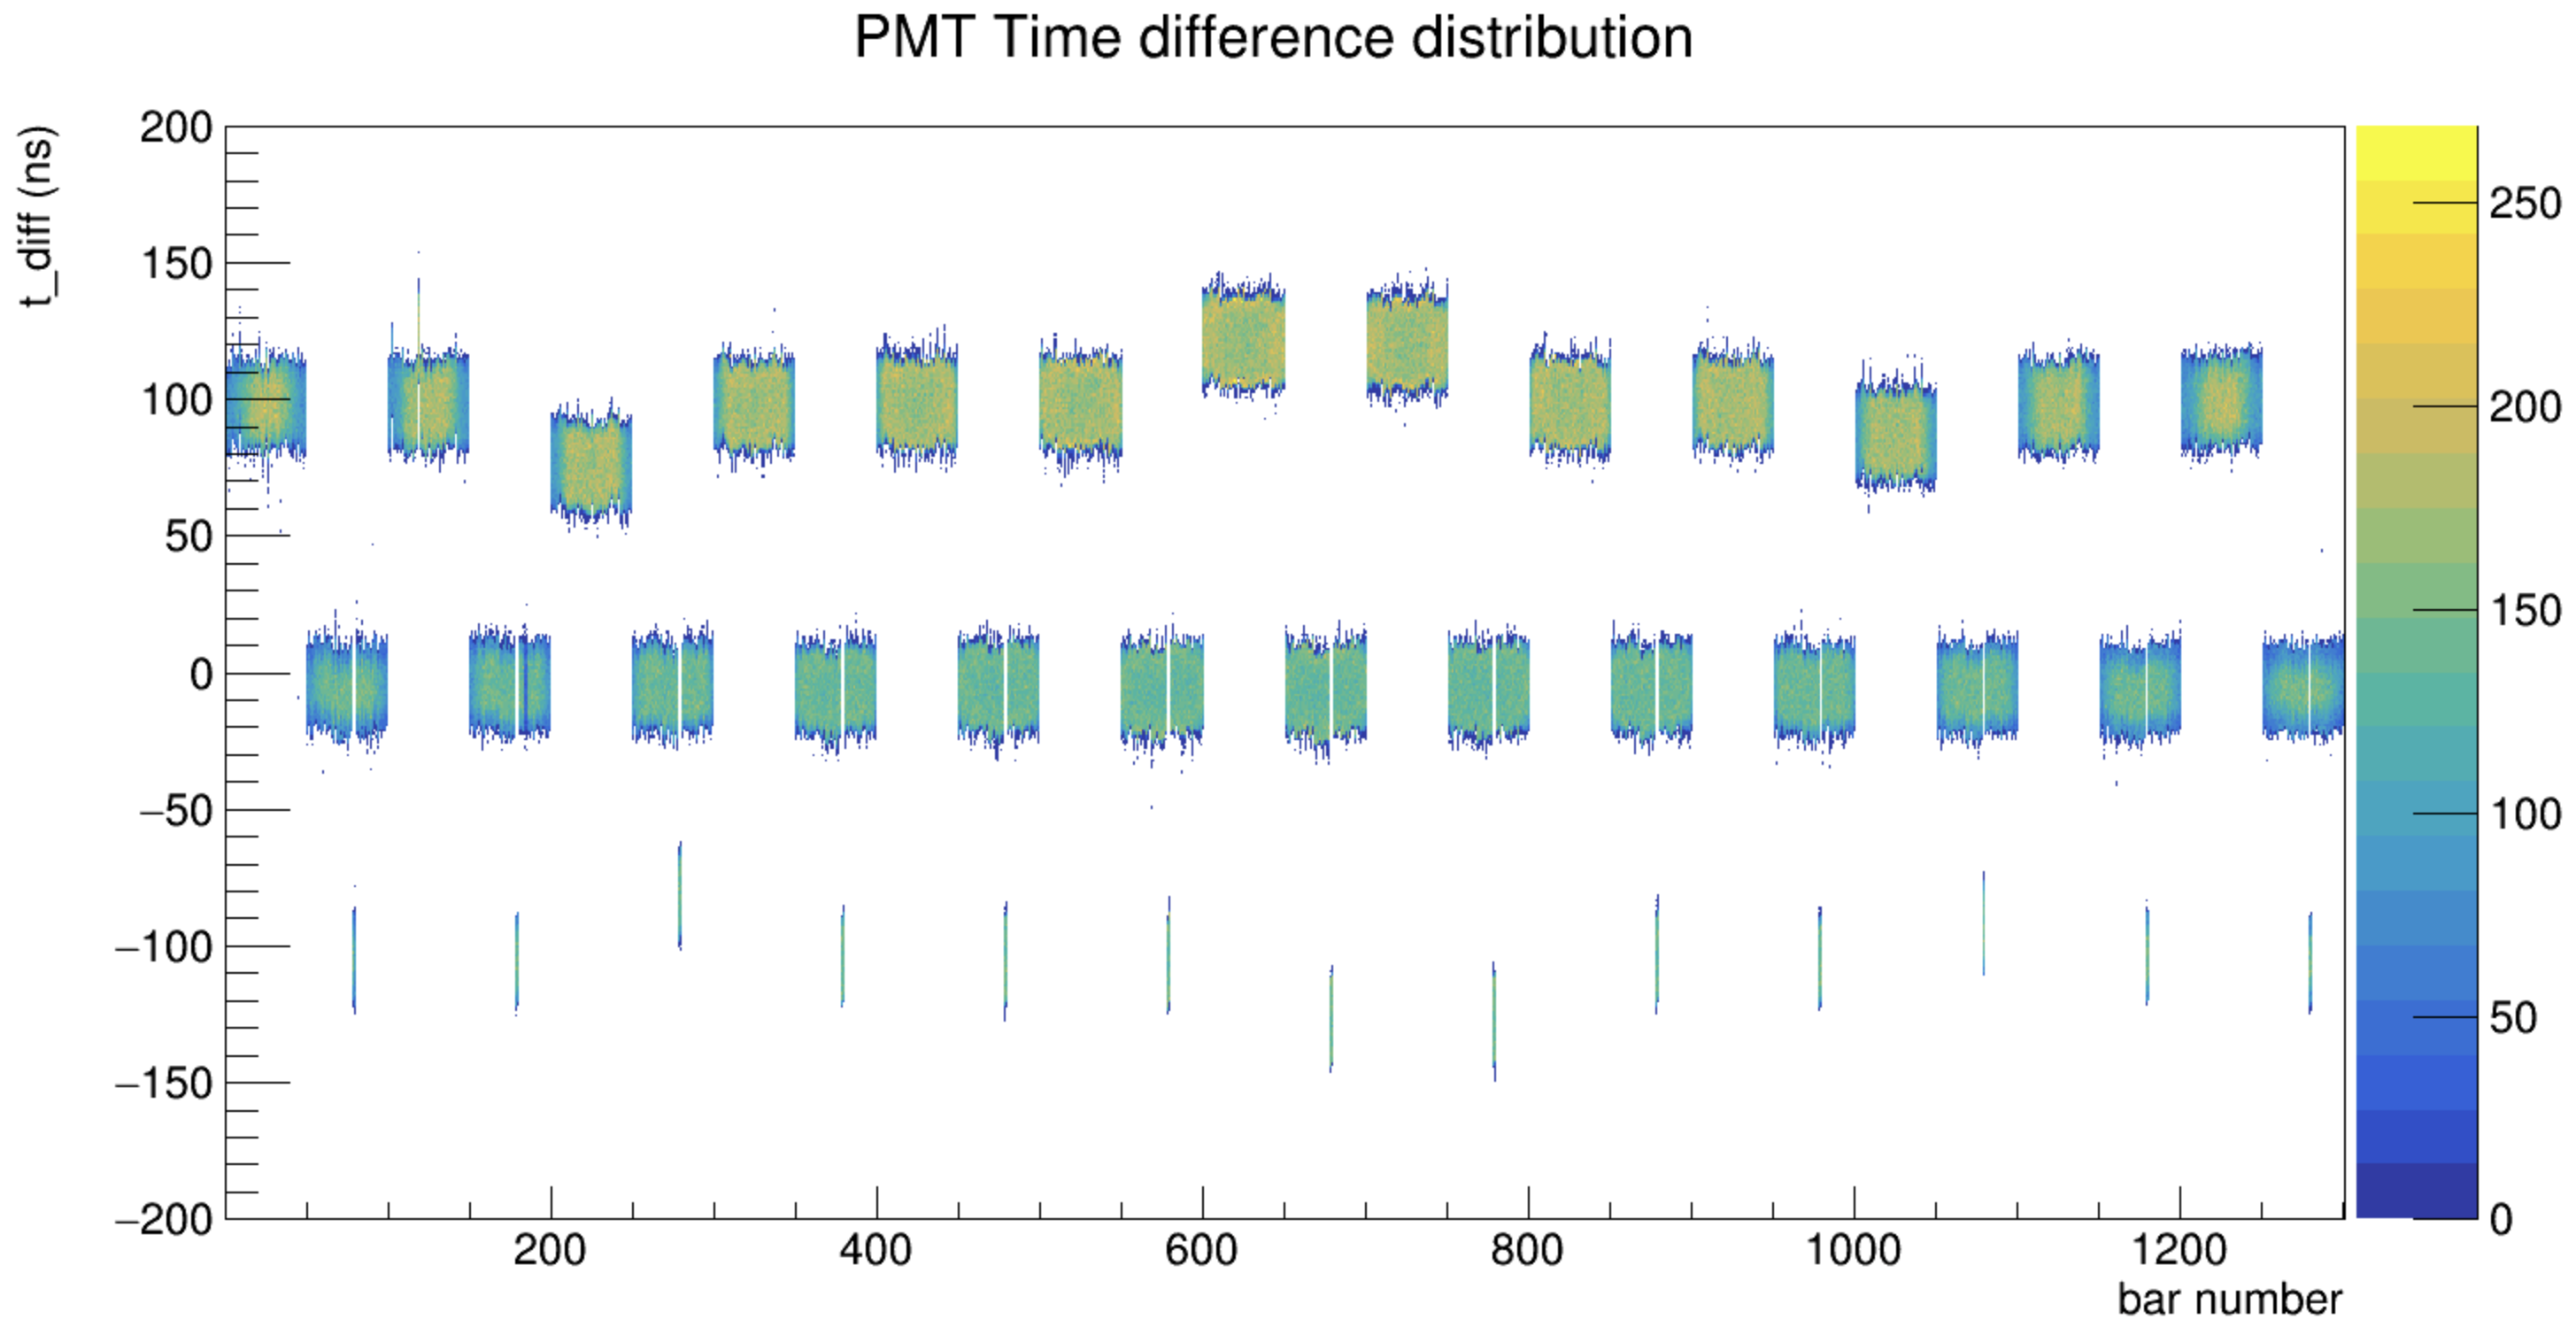
\includegraphics[width = \textwidth]{R3BCon2024GSI/total_tdiff.png}
			\end{figure}
			\vspace{-1em}
			\begin{block}{Calibration steps:}
				\begin{enumerate}
					\setlength\itemsep{0em}
					\small
					\item<1-> Collect time differences of adjacent PMT signals
					\item<2-> Normalize the distribution and convert to the CDF for each bar
					\item<3-> Linear fitting of the CDF within its quantiles of 0.05 to 0.95
				\end{enumerate}
			\end{block}
		\end{column}
		\begin{column}{0.45 \textwidth}
			\begin{figure}
				\captionsetup{singlelinecheck=off,font=footnotesize}
				\caption*{\textit{Parameter fitting:}}
				\vspace*{-0.5em}
				\includegraphics<1>[width = 0.9\textwidth]{neuland/position_cal/TimeDifference2.png}
				\includegraphics<2>[width = 0.9\textwidth]{neuland/position_cal/TimeDifference3.png}
				\includegraphics<3>[width = 0.9\textwidth]{neuland/position_cal/TimeDifference4.png}
			\end{figure}
			\onslide<3->
			{
				\footnotesize
				\setlength{\abovedisplayskip}{0pt}
				\setlength{\belowdisplayskip}{0pt}
				\setlength{\abovedisplayshortskip}{0pt}
				\setlength{\belowdisplayshortskip}{0pt}
				\vspace{-1em}
				\begin{flalign*}
					\intertext{Fitting function:}
					y               & = a \cdot x + 0.5 - a \cdot b       \\
					\intertext{Calculation of parameters:}
					C_e             & = 2 \cdot a \cdot \text{bar length} \\
					t_\text{offset} & = b
				\end{flalign*}
			}
		\end{column}
	\end{columns}
\end{frame}
\end{document}
